\documentclass{VUMIFPSbakalaurinis}
\usepackage{algorithmicx}
\usepackage{algorithm}
\usepackage{algpseudocode}
\usepackage{amsfonts}
\usepackage{amsmath}
\usepackage{bm}
\usepackage{caption}
\usepackage{color}
\usepackage{float}
\usepackage{graphicx}
\usepackage{listings}
\usepackage{subfig}
\usepackage{wrapfig}

\usepackage{enumitem}
\setitemize{noitemsep,topsep=0pt,parsep=0pt,partopsep=0pt}
\setenumerate{noitemsep,topsep=0pt,parsep=0pt,partopsep=0pt}

\hbadness=5000
% Titulinio aprašas
\university{Vilniaus universitetas}
\faculty{Matematikos ir informatikos fakultetas}
\department{Programų sistemų studijų programa}
\papertype{Mokslo tiriamasis darbas II}
\title{Srautinio apdorojimo sistemų balansavimas taikant mašininį mokymąsi}
\titleineng{Balancing stream processing systems using machine learning}
\author{Vytautas Žilinas}
\supervisor{Partn. doc. Andrius Adamonis}
\reviewer{Prof. dr. Aistis Raudys}
\date{Vilnius – \the\year}

% Nustatymai
% \setmainfont{Palemonas}   % Pakeisti teksto šriftą į Palemonas (turi būti įdiegtas sistemoje)
\bibliography{bibliografija}

\begin{document} 
\maketitle

\cleardoublepage\pagenumbering{arabic}
\setcounter{page}{2}

\section{Įvadas}

Šio darbo tikslas - apžvelgti susijusius literatūros šaltinius, pateikti jų santraukas ir panaudoti šią informacija suformuluoti problemą, kuri bus nagrinėjama sekančiame darbe. 

Realaus laiko duomenų apdorojimas (angl. real-time data processing) yra jau senai nagrinėjamas kaip vienas iš būdų apdoroti didelių kiekių duomenis (angl. Big data). Vienas iš realaus laiko apdorojimo sprendimų yra srautinis duomenų apdorojimas. Srautinis duomenų apdorojimas (angl. stream processing) – lygiagrečių programų kūrimo modelis, pasireiškiantis sintaksiškai sujungiant nuoseklius skaičiavimo komponentus srautais, kad kiekvienas komponentas galėtų skaičiuoti savarankiškai \cite{shortstreamproc}. 

Yra keli pagrindiniai srautinio apdorojimo varikliai: „Apache Storm“, „Apache Spark“, „Heron“ ir kiti. „Apache Storm“ ir „Heron“ apdoroja duomenis ne duomenų srautais, o „Apache Spark“ mikro-paketais \cite{karau2015learning}. „Heron“ srautinio apdorojimo variklis, buvo išleistas „Twitter“ įmonės 2016 metais kaip greitesnė alternatyva „Apache Storm“ srautinio apdorojimo varikliui \cite{openSourcing}.Šiame darbe bus naudojamas „Heron“, kadangi tai yra naujesnis ir greitesnis srautinio apdorojimo variklis nei „Apache Storm“ \cite{twitterHeron}. 

Srautinio apdorojimo sistemų balansavimas (angl. auto-tuning) - tai sistemos konfigūracijos valdymas siekiant užtikrinti geriausią resursų išnaudojimą - duomenų apdorojimas neprarandant greičio, bet ir naudojant tik reikiamą kiekį resursų. Kadangi srautinio apdorojimo sistemų komponentai yra kuriami kaip lygiagretus skaičiavimo elementai, todėl jie gali būti plečiami horizontaliai ir vertikaliai \cite{shortstreamproc} keičiant sistemų konfigūraciją. Tačiau lygiagrečių elementų kiekio keitimas nėra vienintelis būdas optimizuoti resursų išnaudojimą. Kiekvienas variklis turi savo rinkinį konfigūruojamų elementų. Darbe naudojamas „Heron“ variklis leidžia optimizuoti sistemas naudojant 56 konfigūruojamus svertus (angl. levers) \cite{configDocument}.

Yra skirtingi būdai kaip gali būti parenkama tinkama konfigūracija. Kadangi dar nėra naudojimui paruoštų sprendimų, kurie galėtų balansuoti srautinio apdorojimo sistemas savarankiškai, dažniausiai tai daro duomenų inžinieriai, kurie dirba su šiomis sistemomis. Kadangi srautinio apdorojimo sistemų apkrovos gali būti skirtingų pobūdžiu (duomenų kiekis, skaičiavimų sudėtingumas, nereguliari apkrova), o inžinieriai konfigūruodami išbando tik keletą derinių ir pasirenka labiausiai tinkanti \cite{selfRegulatingStreaming}, lieka labai daug skirtingų neišbandytų konfigūracijos variacijų. Optimalios konfigūracijos suradimas yra NP sudėtingumo problema \cite{automateTuning}, nes žmonėms yra sunku suvokti didelį kiekį konfigūracijos variacijų. 
Vienas iš būdų automatiškai valdyti konfigūraciją buvo pasiūlytas 2017 metų straipsnyje „Dhalion: self-regulating stream processing in heron“, kuriame autoriai aprašo savo sukurtą sprendimą „Dhalion“, kuris konfigūruoja „Heron“ srautinio apdorojimo sistemas pagal esama apkrova ir resursus, t.y. jei apdorojimo elementų išnaudojimas išauga >100\%, „Dhalion“ padidina lygiagrečiai dirbančių apdorojimo elementų kiekį \cite{dhalion}. Tačiau šis sprendimas leidžia reguliuoti tik elementų lygiagretumą ir tai daro tik reaktyviai.
Vienas iš naujausių būdų balansuoti srautinio apdorojimo sistemas - mašininis mokymasis. Vienas iš tokių bandymų buvo aprašytas 2018 metų straipsnyje „Auto-tuning Distributed Stream Processing Systems using Reinforcement Learning“, kuriame buvo atliktas tyrimas - „Apache Spark“ sistemos balansavimui buvo naudojamas skatinamojo mokymo REINFORCE algoritmas, kuris pagal dabartinę konfigūraciją ir gaunamas metrikas keitė srautinio apdorojimo sistemos konfigūracijas. Šiame tyrime buvo nustatyta, jog sprendimas, naudojantis mašininį mokymąsi, suranda konfigūraciją per trumpesnį laiką nei žmones ir taip pat sukurtą konfigūraciją naudojančios srautinio apdorojimo sistemos laukimo trukme (angl. latency) yra 60-70\% mažesnė nei tyrimo metu žmonių sukurtos konfigūracijos \cite{vaquero2018autotuning}. Šiame darbe naudojamas „Heron“ variklis leidžia prie savęs prijungti sukurtą išorinę metrikų surinkimo programą, kuri gali rinkti tokias sistemų metrikas kaip: naudojama RAM atmintis, CPU apkrova, komponentų paralelizmas ir kitas, kurios bus naudojamos sistemos balansavimui. 

Skatinamasis mokymasis yra vienas iš mašininio mokymosi tipų. Šis mokymasis skiriasi nuo kitų, nes nereikia turėti duomenų apmokymui, o programos mokosi darydamos bandymus ir klysdamos. Pagrindinis uždavinys naudojant skatinamąjį mokymąsi yra surasti balansą tarp naujų sprendimų tyrinėjimo (angl. exploration) ir turimos informacijos išnaudojimo (angl. exploitation) \cite{reinforcment}. Vienas iš pagrindinių privalumų naudojant skatinamąjį mokymąsi balansavimui - nereikia turėti išankstinių duomenų apmokymui kas leidžia jį paprasčiau pritaikyti skirtingoms srautinio apdorojimo sistemų apkrovoms. Tačiau tokio tipo mašininis mokymasis turi ir problemų: sudėtinga aprašyti tinkamos konfigūracijos apdovanojimo (angl. reward) funkciją ir turi būti teisingai aprašytas balansas tarp tyrinėjimo ir išnaudojimo tam, kad nebūtų patirti nuostoliai \cite{selfRegulatingStreaming}.

Yra sukurta daug skatinamojo mokymosi algoritmų (Monte Carl, Q-learning, Deep Q Network ir kiti), tad šiame darbe jie bus apžvelgti ir vienas iš jų bus pasirinktas ir pritaikytas išsikeltam uždaviniui. Algoritmas bus pasirinktas pagal tai, kuris yra tinkamiausias srautinių apdorojimų sistemų balansavimui.

Numatomas magistro darbo tikslas: Ištirti mašininio mokymosi tinkamumą srautinio apdorojimo sistemų balansavimui. 

Numatomi magistro darbo uždaviniai:
\begin{enumerate}
    \item Apibrėžti duomenų pobūdį ir apkrovas, kurios bus naudojamos eksperimente bei pasirinkti srautinio apdorojimo sistemų metrikas, kurios bus naudojamos eksperimento rezultatų palyginimui.
    \item Atlikti literatūros analizė apie esamus skatinamojo mokymosi algoritmus ir pasirinkti vieną iš jų eksperimentui. 
    \item Sukurti eksperimentinį sprendimą, kuris pritaiko pasirinktą mašininio mokymosi algoritmą srautinio apdorojimo sistemų balansavimui.
    \item Atlikti eksperimentą ir palyginti gautus rezultatus su alternatyvomis - „Heron“ su standartine konfigūracija, „Heron“ su „Dhalion“ priedu bei „Heron“ balansavimas pritaikius REINFORCE algoritmą. 
\end{enumerate}


\subsection{Šio darbo tikslas ir uždaviniai}
Tikslas: parengti literatūros apžvalgą, kurioje būtų suformuluota darbe numatoma spręsti problema.

Uždaviniai:
\begin{enumerate}
    \item Išnagrinėti kaip mokslinėje literatūroje matuojamos srautinio apdorojimo sistemos.
    \item Kokius skatinamojo mokymosi algoritmus naudoja kiti autoriai ir kokius rezultatus gauna. 
\end{enumerate}

\section{Srautinio apdorojimo sistemų matavimas ir derinimas}
\subsection{Srautinio apdorojimo sistemos}
Srautinis duomenų apdorojimas (angl. stream processing) – terminas naudojamas apibrėžti sistemas sudarytas iš skaičiavimo elementų (angl. modules) galinčių skaičiuoti lygiagrečiai ir kurios bendrauja kanalais. Tokios sistemų elementai dažniausiai skirstomi į tris klases: šaltinius (angl. sources) kurie paduoda duomenis į sistemą, filtrus (angl. filters) kurie atlieka tam tikrus vienetinius (angl. atomic) skaičiavimus ir nuotakus (angl. sink) kurie perduoda duomenis iš sistemų \cite{stephens1997survey}. 
\begin{figure}[H]
    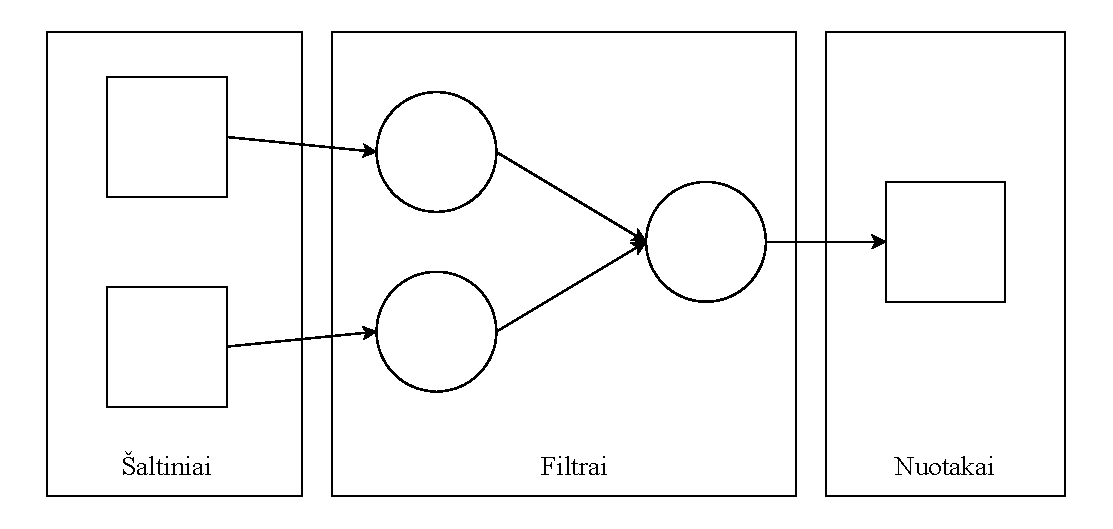
\includegraphics[width=15cm]{img/Srautinio apdorojimo sistema.pdf}
    \caption{Srautinio apdorojimo sistemos pavyzdys}
    \label{srautinio-apdorojimo-sistema}
\end{figure} 
Srautinio apdorojimo sistemos literatūroje yra vaizduojamos orientuotais grafikais (\ref{srautinio-apdorojimo-sistema} pav.). Srautinių apdorojimo sistemos skiriasi nuo reliacinių modelio \cite{babcock2002models}: 
\begin{itemize}
    \item Duomenys į sistemą patenka tinklu, o ne iš fizinių talpyklų.
    \item Duomenų patekimo tvarka negali būti kontroliuojama.
    \item Duomenų kiekis yra neapibrėžtas.
    \item Duomenys apdoroti srautinio apdorojimo sistema yra pašalinami arba archyvuojami, t.y. juos pasiekti yra sunku. 
\end{itemize}
\subsubsection{Duomenų vykdymas}
Srautinio apdorojimo sistemų veikimui reikalingas srautinio apdorojimo variklis (angl. stream processing engine). Šie varikliai yra skirti srautinio apdorojimo sistemų vykdymui, dislokavimui ir užtikrinti plečiamumą (angl. scaling) ir toleranciją gedimams (angl. fault-tolerance) \cite{zhao2017taxonomy}. Populiariųjų srautinio apdorojimo variklių pavyzdžiai: "Apache Storm", "Apache Heron, "Apache Spark", "Apache Samza" ir t.t \cite{roger2019comprehensive}. 
Duomenų vykdymas gali būti išskaidytas į tris komponentus \cite{zhao2017taxonomy}: 
\begin{itemize}
    \item Planavimas (angl. scheduling) - duomenų apdorojimo užduočių planavimas daro įtaką bendram srautinio apdorojimo veikimui \cite{falt2011task}. Pavyzdžiui "Apache Samza" naudoja "Apache YARN" resursų valdymo sistemą, kuri turi planavimo posistemę, kuri skirsto resursus \cite{noghabi2017samza} 
    \item Plečiamumas (angl. scalability) - apibrėžia daug apdorojimo branduolių turinčios sistemos gebėjimą apdoroti didėjanti kiekį užduočių ir galimybę didinti pačią sistemą kad susidoroti su didėjančių kiekiu duomenų \cite{bondi2000characteristics}. Srautinio apdorojimo varikliai turi užtikrinti srautinio apdorojimo sistemų plečiamumą \cite{stonebraker20058}.    
    \item Išskirstytas skaičiavimas (angl. Distributed computation) - tarpusavyje nesusiję skaičiavimo elementai turi naudotojam atrodyti kaip viena darni sistemą \cite{tanenbaum2007distributed}. Srautinio apdorojimo varikliai turi užtikrinti darbų paskirstymą ir skaičiavimo įrenginių koordinacija, kad daug duomenų būtų apdorojami vienu metu \cite{zhao2017taxonomy}.
\end{itemize}
Srautinio apdorojimo sistemos turi viena pagrindinį elementą - srauto procesorių (angl. stream processor), kuris apibrėžia sistemos elementus, aprašo kaip šie sistemos elementai sujungti ir pateikia nustatymus elementams \cite{zhao2017taxonomy}. Pavyzdžiui "Apache Storm" šis elementas vadinimas "topology", kuris yra užrašomas Java kalba naudojant "Apache Storm" pateiktą biblioteką \cite{iqbal2015big}.
\subsubsection{Duomenų priėmimas}
Į srautinio apdorojimo sistemą duomenis patenka per šaltinius, kurie šiuos duomenis perduoda tolimesniems elementams. Dažniausiai duomenis perduodami į sistemą naudojant žinučių eiles (angl. message queues), nes jos turi buferi, kas leidžia mažinti skirtumus tarp duomenų gavimo ir duomenų apdorojimo greičių, ir žinučių eilių brokeriai gali atfiltruoti duomenis ir nukreipti juos į tinkamus šaltinius \cite{kamburugamuve2016survey}. Tačiau šaltiniai turi turėti galimybę rinkti išsaugotus ir priimti ateinančius naujus duomenis \cite{stonebraker20058}, todėl nors ir šaltiniai dažniausiai priima srautinius duomenis, jie turi taip pat gebėti naudoti duomenis iš talpyklų \cite{zhao2017taxonomy}. 

\subsection{Srautinio apdorojimo sistemų matavimas}
Svarbiausias srautinio apdorojimo sistemų reikalavimas - duomenų apdorojimas ir rezultatų grąžinimas turi būti be atsilikimo - didelių apimčių srautiniai duomenys turi būti apdorojami taip pat greitai kaip ateiną \cite{stonebraker20058}. 

\subsubsection{Srautinio apdorojimo sistemų metrikos}
Kitų autorių naudojamos metrikos:
\begin{itemize}
    \item Pralaidumas (angl. Throughput) - per tam tikrą laiko tarpą apdorojamų įvykių kiekis. Kuo didesnis pralaidumas tuo greitaveiką didesnė. 
    \item Gaišaties laikas (angl. Latency) - laiko intervalas nuo apdorojimo arba įvykio pradžios iki apdorojimo pabaigos. Kuo jis mažesnis tuo greitaveiką didesnė.
\end{itemize}
Gaišaties laikas ir pralaidumas dažniausiai nekoreliuoja - sistemos kurios apdoroja srautus paketais turi didesnį pralaidumą, tačiau laikas per kurį renkamas paketas duomenų paveikia laiką kada duomenis patenka į apdorojimo sistemą \cite{Karimov2018BenchmarkingDS}. \par

\cite{stonebraker20058} straipsnyje minima, jog srautinio apdorojimo sistemos naudotojas turi išbandyti savo sistemą su tiksliniu darbo krūviu ir išmatuoti pralaidumą ir gaišaties laiką. \cite{Karimov2018BenchmarkingDS} lyginą srautinio apdorojimo variklius ir matavimui naudoja gaišaties laiką, kurį išskaido į įvykio gaišaties laiką (angl. event-time latency) - laiko intervalas nuo įvykio laiko iki rezultato gavimo iš srautinio apdorojimo sistemos ir apdorojimo gaišaties laiką (angl. processing-time latency) - laiko intervalas nuo duomens patekimo į srautinio apdorojimo sistemą iki rezultato grąžinimo. Šį skaidymą autoriai daro, nes vertinant sistemas dažnai ignoruojamas įvykio laikas ir gaunamas daug mažesnis gaišaties laikas negu jis iš tikro yra. Taip pat autoriai išskiria darnų pralaidumą (angl. sustainable throughput) - didžiausia apkrova įvykių, kurią sistema gali apdoroti be pastoviai augančio įvykio gaišaties laiko, todėl savo eksperimentuose autoriai užtikrina kad duomenų generavimo greitis atitiktų sistemos darnų pralaidumą. Tam kad sužinoti darnų pralaidumą sistemos autoriai pradeda leisti labai didelį srautą duomenų ir mažina iki kol sistemos apdorojimas palaiko generavimo greičius. Visus gaišaties laiko rezultatus autoriai pateikia maksimalaus pralaidumo apdorojimo ir 90\% pralaidumo apdorojimo vidurkiu, minimumu, maksimumu, kvantiliais (90, 95, 99). \cite{hirzel2014catalog} autoriai nagrinėja srautiniam apdorojimui galimas optimizacijas ir matavimui naudoja normalizuotą pralaidumą (naudojamas vienetas kaip vidurkis), nes tai leidžia lengviau palyginti santykinę greitaveiką. Taip pat \cite{hirzel2014catalog} pastebi, kad nors ir yra daug metrikų, kuriomis galima matuoti optimizaciją: pralaidumas, gaišaties laikas, paslaugos kokybė (angl. quality of service), energijos ir tinklo panaudojimas, tačiau pagerinus pralaidumą pagerėja ir visos kitos metrikos. \cite{Qian2016Benchmarking} srautinių apdorojimo sistemų matavimui naudoja pralaidumą (skaičiuojamą baitais per sekundę) ir gaišaties laiką, kaip vidurkį nuo duomens patekimo į sistemą iki apdorojimo pabaigos. Taip pat kadangi autoriai lyginą srautinio apdorojimo variklius jie įveda metriką gedimo toleravimo (angl. fault tolerance) vertinimui, kuriam autoriai išjungia tam tikrą kiekį elementų ir matuoja pralaidumą ir gaišaties laiką. \cite{zhang2020heron} palyginimui naudoja sistemos įvykdymo gaišaties laiką (angl. system completion latency), kuris parodo vidutinį laiko tarpą per kurį kortežas nukeliauja nuo šaltinio iki sistemos galutinio taško. Autoriai skaičiavo vidutinį laiką 5 sekundes intervalais. 
Taip pat autoriai naudojo matavimui CPU apkrovą kiekvienos instancijos (angl. instance), CPU apkrovą kiekvieno darbinio mazgo (angl. worker node) ir apkrovą tarp instancijų/tarp mazgų, kadangi jų užduotis buvo patobulinti esamą planavimo posistemę.  \cite{dhalion} matuoja pralaidumą per minutę. \cite{vaquero2018autotuning} tyria labai panašią problemą - srautinių apdorojimo sistemų balansavimą taikant skatinamąjį mokymą ir matavimui naudoja 99 kvantilį gaišaties laiko. \cite{Chintapalli2016Benchmarking} naudoja gaišaties laiko srautinio apdorojimo variklių vertinimui.

\subsubsection{Srautinio apdorojimo sistemos pobūdis}

Srautinio apdorojimo sistemos gali turėti labai skirtingą elementų išsidėstymą ir nuo to priklauso jų greitaveiką. \cite{Karimov2018BenchmarkingDS} matavimui naudojo du filtrus - agregavimo, kuris skaičiavo visus pirkimus ir jungimo (angl. join) kuris skaičiavo duomenis pagal tam tikrą bendrą rodiklį iš abiejų duomenų srautų. \cite{Qian2016Benchmarking} srautinio apdorojimo variklių palyginimui naudoja septynis skirtingus uždavinius. Vienas iš jų yra WordCount uždavinys, kuris yra plačiai priimtas kaip didelių duomenų apdorojimo sistemos matavimo standartas \cite{huang2010hibench}. Šis uždavinys susidaro iš dviejų elementų: pirmas padalina teksto eilutę į žodžius, antras agreguoja kiekvieno žodžio bendra skaitiklį ir atnaujina bendrą rezultatą žodžių dažnio, kur raktas tai žodis, o reikšmė tai kiek kartojosi šis žodis (\ref{wordcount} pav.). 
\begin{figure}[H]
    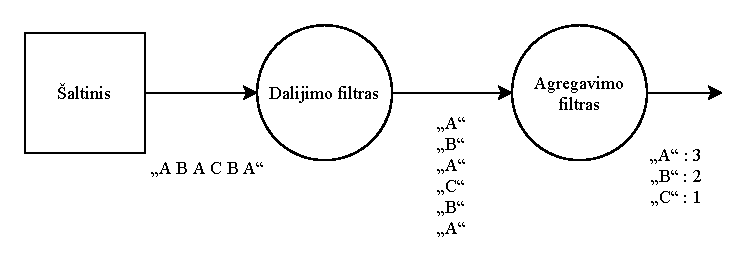
\includegraphics[width=15cm]{img/wordcount.pdf}
    \caption{WordCount sistemos pavyzdys}
    \label{wordcount}
\end{figure} 
\cite{zhang2020heron}  matavimui naudoja WordCount sistemą, kuri yra paprastesnė, nei \ref{wordcount} pav., nes šaltinis generuoja ir siunčia po vieną žodį ir yra tik agregavimo filtras, ir naudoja SentenceWordCount sistemą, kuri yra identiška \ref{wordcount} pav. pavaizduotai sistemai. Taip pat autoriai sukūrė FileWordCount sistemą, kuri atlieką tą patį kaip ir SentenceWordCount, tačiau šaltinis ne pats generuoja žodžius, o skaito iš tekstinio dokumento ir taip pat naudojo egzistuojančią Yahoo srautinio apdorojimo vertinimą (angl. benchmarking) \cite{Chintapalli2016Benchmarking}. \cite{dhalion} naudojo WordCount eksperimentui. \cite{vaquero2018autotuning} eksperimentams naudojo Yahoo srautinio apdorojimo palyginimą \cite{Chintapalli2016Benchmarking} ir taip pat darė bandymus su realiais daiktų interneto (angl. internet of things) įmonės duomenimis. \cite{Chintapalli2016Benchmarking} apibrėžia srautinio apdorojimo sistemą vertinimui skirtingu srautinio apdorojimo variklių. Ši sistemą analizuoja reklamas pagal tipą ir matomumą ir rezultatus deda į Redis duomenų bazę. Sistema sukurta taip, kad aprėptu visas srautinio apdorojimo sistemos savybes (\ref{yahoo} pav.).
\begin{figure}[H]
    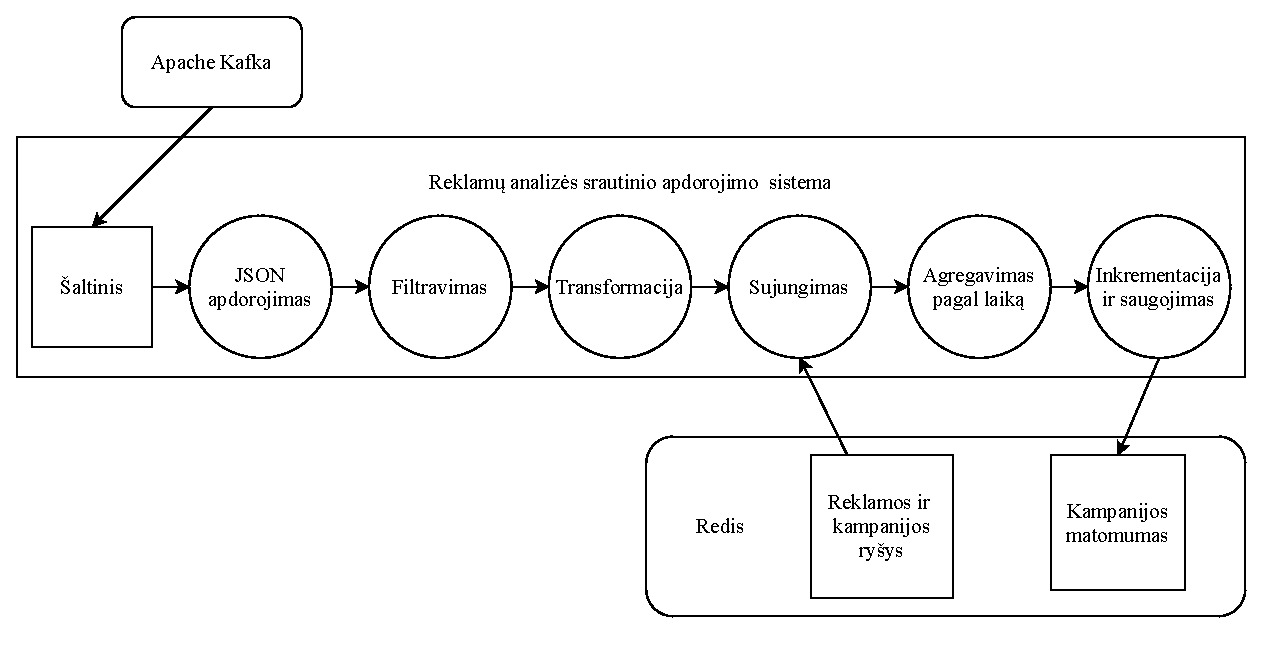
\includegraphics[width=15cm]{img/yahoo.pdf}
    \caption{Reklamų analizės sistema \cite{Chintapalli2016Benchmarking}}
    \label{yahoo}
\end{figure} 

\subsubsection{Srautinio apdorojimo sistemų matavimo duomenys}

Vertinant sistemų greitaveiką reikia atsižvelgti ir į testavimui naudojamus duomenis. \cite{Karimov2018BenchmarkingDS} naudoja žaidimų kūrimo įmonės Rovio duomenis ir naudoja du duomenų srautus - pirkimo srautas kur siunčiami kortežai (angl. tuples) susidarantys iš nupirktos valiutos kiekio, laiko ir naudotojo kuris nupirko ir reklamų srautas kuris siunčia nagrinėja valiutos pirkimo siūlymus tam tikru laiku. Generuojami duomenis naudojant normalizuotą paskirstymą ant raktinio lauko. \cite{Qian2016Benchmarking} naudoja tekstinius duomenis iš AOL paieškos variklio ir apdoroja juos pagal pasirinktus uždavinius. \cite{zhang2020heron} matavimui naudoja šaltinių generuojamą tekstą, kadangi lyginamas tas pats srautinio apdorojimo variklis tik su pakeista planavimo posisteme ir naudoja iš anksto sugeneruotą tekstą patalpintą į tekstinį dokumentą. \cite{Chintapalli2016Benchmarking} aprašo sistemą kuri daro skirtingų srautinio apdorojimo variklių palyginimus.  
Šiam vertinimui naudojami duomenys simuliuojantys reklamas. Autoriai naudoja savo duomenų generatorių.

\subsection{Srautinio apdorojimo sistemų derinimas}
Sistemų greitaveika yra tiesiogiai susijusi su konfigūravimo parametrais, kurie valdo tokius aspektus kaip atminties valdymas, gijų skaičius, planavimas, resursų valdymas \cite{lu2019speedup}. Taip pat yra išnagrinėta, jog neteisingi nustatymai turi nuostolingus efektus ant sistemos greitaveikos ir stabilumo \cite{herodotou2011starfish}. 

\cite{herodotou2020survey} išskiria 3 pagrindinius automatinio derinimo iššūkius:
\begin{enumerate}
    \item Didelė ir sudėtinga parametrų erdvė - "Apache Spark" ir "Apache Storm" turi virš 150 konfigūruojamų parametrų \cite{Bilal2017Towards, petridis2016spark}. Taip pat kai kurios nustatymų reikšmės, kurios tinka vienam uždaviniu, gali turėti neigiamos įtakos kitam \cite{herodotou2011starfish, Pooyan2016Uncertainty}.
    \item Sistemų mastas ir sudėtingumas - Sistemų administratoriai turi gebėti konfigūruoti didelius kiekius skaičiavimo mazgų, kurie gali skirtis CPU, atmintimi, tinklo tipais \cite{herodotou2020survey}.
    \item Pradinių duomenų statistikos trūkumas - įvedimo duomenys srautinėse apdorojimo sistemose yra realus srautai, kurie stipriai varijuoja savo apimtimi \cite{Dayarathna2018Recent}.
\end{enumerate}  

\cite{Trotter2017Into} nagrinėjantis tinkamos konfigūracijos radimą naudojant genetinius algoritmus "Apache Storm" srautinio apdorojimo sistemoms nustatė, jog lygiagretumo laipsnis labiausiai daro įtaką srautinio apdorojimo sistemų greitaveikai. 
"Apache Heron" yra srautinio apdorojimo variklis, kuris sukurtas pagal "Apache Storm" su patobulinimais \cite{twitterHeron} pateikia naują būdą kontroliuoti srautą - priešslėgis (angl. backpressure), kuris leidžia filtrui sulėtinti prieš jį einantį elementą, kas leidžia sumažinti gaišaties laiką ir taip pat gali būti naudojamas kaip greitaveikos praradimo indikatorius \cite{bansal2018trevor}.
Taip pat \cite{bansal2018trevor} nagrinėja "Apache Heron" automatinį konfigūravimą naudojant iš anksto aprašytas taisykles. 


\section{Skatinamojo mokymosi algoritmai}
\cite{herodotou2020survey} aprašo skirtingus sprendimus automatiniam konfigūravimui ir išskiria šiuos mašininio mokymosi privalumus:
\begin{itemize}
    \item Nebūtina suprasti sistemos, užduočių ir duomenų, kadangi naudojamas juodos dėžės (angl. black-box) principas.
    \item Mašininio mokymosi modelis pats save tobulina, kuo daugiau gauna duomenų. 
\end{itemize}
Šio straipsnio autoriai išskiria mašininio mokymosi iššūkius : 
\begin{itemize}
    \item Parametrų parinkimas - kadangi konfigūruojamų parametrų kiekis yra didelis \cite{Bilal2017Towards, petridis2016spark} ne visi iš jų stipriai daro įtaką greitaveikai, todėl pirma išsirinkti aktualiausius parametrus resursų valdymo, užduočių planavimo ir duomenų valdymo. Tam dažnai naudojama eksperto pagalba \cite{wang2016novel}, gidai arba eksperimentavimo pagalba. Tačiau galima ir naudoti mašininio mokymosi algoritmą, kad nustatyti koreliacija tarp parametrų ir greitaveikos \cite{vaquero2018autotuning, yang2012statistics}
    \item Mašininio mokymosi modelio pasirinkimas - kadangi yra nemažai skirtingų mašininio mokymosi metodų kurie tinka derinimo uždaviniui.
\end{itemize} 
Taip pat pateikiami pavyzdžiai paketinio apdorojimo ir srautinio apdorojimo derinimo naudojant mašininį mokymąsi straipsniai (\ref{ml-in-stream} lentelėje pateikiami tik išrinkti srautinio apdorojimo pavyzdžiai).

\begin{table}[H]
    \begin{tabular}{|l|p{0.42\textwidth}|p{0.25\textwidth}|}
    \hline
    Būdas    & Įvesties savybės                                                                    & Mašininio mokymosi metodai                 \\ \hline
    Zacheilas et al. \cite{zacheilas2015elastic}  & Rinkinys kelių konfigūracijos parametrų                                             & Gaussian Processes                         \\ \hline
    Li et al. \cite{li2016performance}         & Atminties dydžiai ir branduolių ir gijų kiekis skirtingose stadijose                & Support Vector Regression                  \\ \hline
    Trotter et al. \cite{Trotter2017Into}  & Darbinių procesų kiekis, vykdytojų kiekis                                           & Genetic Algorithm, Bayesian Optimization   \\ \hline
    Trotter et al. \cite{trotter2019forecasting} & Vykdytojai, šaltinių ir filtrų lygiagretumas, acker lygiagretumas                   & Genetic Algorithm, Support Vector Machines \\ \hline
    OrientStream \cite{wang2017automating}    & Įvairios duomenų, plano, filtrų ir klasterio lygio savybės                       & Ensemble/Incremental ML                    \\ \hline
    Vaquero et al. \cite{vaquero2018autotuning} & Parametrai ir metrikos parinkti faktorinės analizės (angl. factor analysis) pagalba & Reinforcement Learning                     \\ \hline
    \end{tabular}
    \caption{Srautinių sistemų derinimo naudojant mašininį mokymąsi pavyzdžiai}
    \label{ml-in-stream}
    \end{table}
\printbibliography[heading=bibintoc] 

\end{document}
